\documentclass{article}
\usepackage[left=3cm,right=3cm,top=2cm,bottom=2cm]{geometry} % page settings
\usepackage{amsmath} % provides many mathematical environments & tools
\usepackage{graphicx}
\usepackage{mathrsfs}

\setlength{\parindent}{0mm}
\makeatletter
\setlength{\@fptop}{0pt}
\makeatother


\newcommand{\RNum}[1]{\uppercase\expandafter{\romannumeral #1\relax}}


\begin{document}

\title{CSE 250A: Assignment 2}
\author{Jiaxu Zhu}
\date{\today}
\maketitle
%%%%%%%%%%%%%%%%%%%%%%%%%%%%%%%%%%%%%%%%%%%%%%%%%%%%%%%%%%%%%%%%%%%%%%%%%%%%%%%%%%%%%%%%%%%
\subsection*{2.1 Probabilistic inference}
\subsubsection*{(a)}

\begin{eqnarray*}
	P(A=1|E=1) & = & P(A=1|E=1,B=0)P(B=0) + P(A=1|E=1,B=1)P(B=1) = 0.2907\\
	P(A=1|E=0) & = & P(A=1|E=0,B=0)P(B=0) + P(A=1|E=0,B=1)P(B=1) = 0.0019\\
	P(A=1) & = & P(A=1|E=1)P(E=1) + P(A=1|E=0)P(E=0) = 0.0025\\
	P(E=1|A=1) &=& \frac{P(A=1|E=1)P(E=1)}{P(A=1)} = 0.2326\\
\end{eqnarray*} 

\subsubsection*{(b)}

\begin{eqnarray*}
	P(A=1|B=1) & = & P(A=1|B=1,E=0)P(E=0) + P(A=1|B=1,E=1)P(E=1) = 0.94\\
	P(E=1|A=1,B=1) &=& \frac{P(A=1|E=1,B=1)P(E=1|B=1)}{P(A=1|B=1)} = 0.002\\
\end{eqnarray*}

\subsubsection*{(c)}

\begin{eqnarray*}
P(J=1) &=& P(J=1|A=1)P(A=1)+P(J=1|A=0)P(A=0) = 0.0521\\
P(A=1|J=0) &=& \frac{P(J=0|A=1)P(A=1)}{P(J=0)} = 0.0003\\
\end{eqnarray*}

\subsubsection*{(d)}

\begin{eqnarray*}
	P(A=1|J=0,M=0) &=& \frac{P(J =0,M =0|A=1)P(A=1)}{P (J = 0, M = 0)}\\
	&=& \frac{P(J =0|A=1)P(M =0|A=1)P(A=1)}{\sum_{a}P(J =0|A=a)P(M =0|A=a)P(A=a)}~~(marginalization \& d-separation \RNum{3})\\
	&=& 0.00008\\
\end{eqnarray*}

\subsubsection*{(e)}

\begin{eqnarray*}
	P(M=1) &=& P(M=1|A=1)P(A=1)+P(M=1|A=0)P(A=0) = 0.0117\\
	P(A=1|M=1) &=& \frac{P(M=1|A=1)P(A=1)}{P(M=1)} = 0.1500\\
\end{eqnarray*}

\subsubsection*{(f)}

\begin{eqnarray*}
	P (A = 1|M = 1, E = 0) &=& \frac{P (M = 1, E = 0|A = 1)P (A = 1)}{P (M = 1, E = 0)}\\
	&=& \frac{P(M = 1|A = 1)P(E = 0|A = 1)P(A = 1)}{􏰄a P (M = 1|A = a)P (E = 0|A = a)P (A = a)}~~(marginalization \& d-separation \RNum{3})\\
	&=& 0.1197\\
\end{eqnarray*}

Results seem consistent with commonsense patterns of reasoning by one factor explaining away another one.

%%%%%%%%%%%%%%%%%%%%%%%%%%%%%%%%%%%%%%%%%%%%%%%%%%%%%%%%%%%%%%%%%%%%%%%%%%%%%%%%%%%%%%%%%%%
\subsection*{2.2 Probabilistic reasoning}

\subsubsection*{(a)}
First, we compute the $P(D|S_1=1,...,S_k=1)$ as a function of $k$.
\begin{eqnarray*}
	P(D|S_1=1,S_2=1...,S_k=1) &=& \frac{P(S_1=1,S_2=1...,S_k=1|D)P(D)}{P(S_1=1,S_2=1...,S_k=1)}\\
	&=& \frac{\prod_{i=1}^{k}P(S_i|D)P(D)}{P(S_1=1,S_2=1...,S_k=1)}~~(d-separation~~\RNum{3})
\end{eqnarray*}

then we have
\begin{eqnarray*}
	r_k &=& \frac{P(D=0|S_1=1,S_2=1...,S_k=1)}{P(D=1|S_1=1,S_2=1...,S_k=1)}\\
	&=&\frac{\prod_{i=1}^{k}P(S_i|D=0)}{\prod_{i=1}^{k}P(S_i|D=1)}\\
	&=&\frac{2^k}{2^k+(-1)^k}
\end{eqnarray*}

for $k$ as odd numbers, $r_k = \frac{2^k}{2^k-1} > 1$, the first form of the disease will be diagnosed; for $k$ as odd numbers, $r_k = \frac{2^k}{2^k+1} < 1$, the second form of the disease will be diagnosed.

\subsubsection*{(b)}

As showed in (a) above, two form of the disease will be diagnosed alternatively according to the parity of $k$. Thus, the diagnosis dosen't become more or less certain as more symptoms are observed. The form of disease D are uniformly likely to be observed instead.

\subsection*{Sigmoid function}
\subsubsection*{(a)}
\begin{eqnarray*}
	\sigma'(z) &=& -\frac{1}{(1+e^{-z})^2} \times (-e^{-z}) \\
		&=& \frac{1}{1+e^{-z}} \times \frac{e^{-z}}{1+e^{-z}} \\
		&=& \frac{1}{1+e^{-z}} \times \frac{1}{1+e^{z}} \\
		&=& \sigma(z) \sigma(-z)
\end{eqnarray*}

\subsubsection*{(b)}
\begin{eqnarray*}
	\sigma(-z) + \sigma(z) &=&  \frac{1}{1+e^{z}} + \frac{1}{1+e^{-z}}\\
	&=& \frac{1}{1+e^{z}} + \frac{e^z}{1+e^z}\\
	&=& 1
\end{eqnarray*}

\subsubsection*{(c)}
\begin{eqnarray*}
	L(\sigma(z)) &=& \log(\frac{\sigma(z)}{1-\sigma(z)})\\
	&=& \log(\frac{\frac{1}{1+e^{-z}}}{1-\frac{1}{1+e^{-z}}})\\
	&=& \log(e^z)\\
	&=& z
\end{eqnarray*}


%%%%%%%%%%%%%%%%%%%%%%%%%%%%%%%%%%%%%%%%%%%%%%%%%%%%%%%%%%%%%%%%%%%%%%%%%%%%%%%%%%%%%%%%%%%
\subsection*{2.4 Conditional independence}

\begin{table}[h!]
	\centering
	\begin{tabular}{|p{2cm}|p{2cm}|p{4cm}|}
		\hline
		X & Y & E \\
		\hline
		month & water & sprinkler, rain\\
		\hline
		month & water & sprinkler, rain, fall\\
		\hline
		month & fall & sprinkler, rain\\
		\hline
		month & fall & water\\
		\hline
		month & fall & water, sprinkler\\
		\hline
		month & fall & water, rain\\
		\hline
		month & fall & water, sprinkler, rain\\
		\hline
		sprinkler & rain & month \\
		\hline
		sprinkler & fall & water \\
		\hline
		sprinkler & fall & water, month \\
		\hline
		sprinkler & fall & water, rain\\
		\hline
		sprinkler & fall & water, month, rain \\
		\hline
		rain & fall & water \\
		\hline
		rain & fall & water, month \\
		\hline
		rain & fall & water, sprinkler\\
		\hline
		rain & fall & water, month, sprinkler \\
		\hline
	\end{tabular}
	\caption{Question 2.4}
\end{table}


%%%%%%%%%%%%%%%%%%%%%%%%%%%%%%%%%%%%%%%%%%%%%%%%%%%%%%%%%%%%%%%%%%%%%%%%%%%%%%%%%%%%%%%%%%%

\subsection*{2.5 Markov blanket}
\begin{figure}[h!]
	\centering
	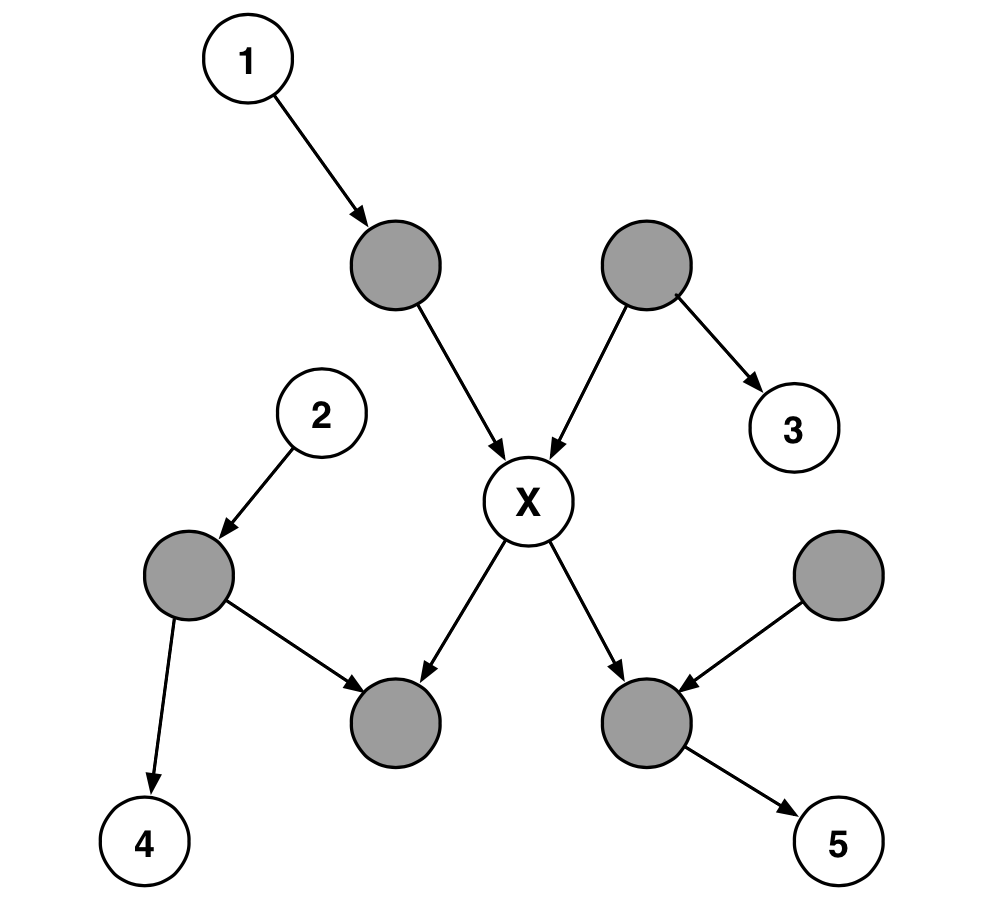
\includegraphics[width=8cm]{q2.5.png}
	\caption{Five Possible Paths}
	\label{path}
\end{figure}

For any node $Y$, satisfying $Y \notin B_X$ and $Y \notin X$, there only exist five different kinds of paths from $Y$ to $X$:

\begin{enumerate}
	\item
	Through the parents of its parents (denoted as node 1 in Fig.\ref{path}); Then this path is 'd-separated' due to rule \RNum{1};
	\item
	Through the parents of its children's parents (denoted as node 2 in Fig.\ref{path}); Then this path is 'd-separated' due to rule \RNum{1};
	\item
	Through the children of its parents (denoted as node 3 in Fig.\ref{path}); Then this path is 'd-separated' due to rule \RNum{2};
	\item
	Through the children of its children's parents (denoted as node 4 in Fig.\ref{path}); Then this path is 'd-separated' due to rule \RNum{2};
	\item
	Through the children of its children (denoted as node 5 in Fig.\ref{path}); Then this path is 'd-separated' due to rule \RNum{1}.
\end{enumerate}

Above all, we can say that 
\begin{eqnarray*}
	P(X,Y|B_X) = P(X|B_X)P(Y|B_X)
\end{eqnarray*}

%%%%%%%%%%%%%%%%%%%%%%%%%%%%%%%%%%%%%%%%%%%%%%%%%%%%%%%%%%%%%%%%%%%%%%%%%%%%%%%%%%%%%%%%%%%
\subsection*{2.6 Noisy-OR}
\begin{eqnarray*}
	P(Z=1|X=0,Y=0) & < & P(Z=1|X=0,Y=1)\\
	P(Z=1|X=1,Y=0) & < & P(Z=1|X=0,Y=1)\\
	P(Z=1|X=1,Y=0) & < & P(Z=1|X=1,Y=1)\\
	P(X=1) & < & P(X=1|Z=1)\\
	P(X=1) & = & P(X=1|Y=1)\\
	P(X=1|Z=1) & > & P(X=1|Y=1,Z=1)\\
	P(X=1)P(Y=1)P(Z=1) & < & P(X=1, Y=1, Z=1)
\end{eqnarray*}





%%%%%%%%%%%%%%%%%%%%%%%%%%%%%%%%%%%%%%%%%%%%%%%%%%%%%%%%%%%%%%%%%%%%%%%%%%%%%%%%%%%%%%%%%%%
\subsection*{2.7 More conditional independence}

\begin{table}[h!]
	\centering
	\begin{tabular}{|p{8cm}|p{2cm}|}
		\hline
		statements & independence?\\
		\hline
		$P(E,F|D) = P(E|D)P(F|D) $ & False \\
		\hline
		$P(E,F|C,D) = P(E|C,D)P(F|C,D) $ & False \\
		\hline
		$P(E,F|A,B,D) = P(E|A,B,D)P(F|A,B,D) $ & True \\
		\hline
		$P(D|C) = P(D)$ & False \\
		\hline
		$P(D|A,B) = P(D|A,B,C)$ & True \\
		\hline
		$ P(A,B) = P(A)P(B) $ & True \\
		\hline
		$P(A|C,D) = P(A|C,D,F)$ & False \\
		\hline
		$P(A|B,C,D) = P(A|B,C,D,F)$ & True \\
		\hline
		$P(B|A,C,D,F) = P(B|A,C,D,F,E)$ & True \\
		\hline
		$P(B,F,A,E|C,D) = P(B,F|C,D)P(A,E|C,D)$ & False \\
		\hline
	\end{tabular}
	\caption{Question 2.7}
\end{table}

\subsection*{2.8 Even more conditional independence}

\begin{table}[h!]
	\centering
	\begin{tabular}{|p{6cm}|p{4cm}|}
		\hline
		$P(B|D) = P(B|\mathcal{S})$ & $\mathcal{S}=\{A,C,D,E,G\}$\\
		\hline
		$ P(B|D,F) = P(B|\mathcal{S})$ & $\mathcal{S}=\{D,F,G\}$ \\
		\hline
		$ P(C|D) = P(C|\mathcal{S})$ & $\mathcal{S}=\{B,D,G\}$ \\
		\hline
		$ P(C|F,G) = P(C|\mathcal{S}) $ & $\mathcal{S}=\{F,G\}$\\
		\hline
		$P(C|A,E,F) = P(C|\mathcal{S})$ & $\mathcal{S}=\{A,E,F\}$\\
		\hline
		$ P(E|F) = P(E|\mathcal{S}) $ & $\mathcal{S}=\{F\}$\\
		\hline
		$P(E|C) = P(E|\mathcal{S}) $ & $\mathcal{S}=\{A,B,C,D,F,G\}$\\
		\hline
		$P(F) = P(F|\mathcal{S})$ & $\mathcal{S}=\emptyset$\\
		\hline
		$ P(F|C,D) = P(F|\mathcal{S})$ & $\mathcal{S}=\{C,D,E,G\}$\\
		\hline
        $ P(A,B) = P(A,B|\mathcal{S}) $ & $\mathcal{S}=\emptyset$\\
        \hline
	\end{tabular}
	\caption{Question 2.8}
\end{table}

\end{document}

